\documentclass[a4paper,12pt]{article}
%%%%%%%%%%%%%%%%%%%%%%%%%%%%%%%%%%%%%%%%%%%%%%%%%%%%%%%%%%%%%%%%%%%%%%%%%%%%%%%%%%%%%%%%%%%%%%%%%%%%%%%%%%%%%%%%%%%%%%%%%%%%%%%%%%%%%%%%%%%%%%%%%%%%%%%%%%%%%%%%%%%%%%%%%%%%%%%%%%%%%%%%%%%%%%%%%%%%%%%%%%%%%%%%%%%%%%%%%%%%%%%%%%%%%%%%%%%%%%%%%%%%%%%%%%%%
\usepackage{eurosym}
\usepackage{vmargin}
\usepackage{amsmath}
\usepackage{graphics}
\usepackage{framed}
\usepackage{epsfig}
\usepackage{subfigure}
\usepackage{fancyhdr}

\setcounter{MaxMatrixCols}{10}
%TCIDATA{OutputFilter=LATEX.DLL}
%TCIDATA{Version=5.00.0.2570}
%TCIDATA{<META NAME="SaveForMode"CONTENT="1">}
%TCIDATA{LastRevised=Wednesday, February 23, 201113:24:34}
%TCIDATA{<META NAME="GraphicsSave" CONTENT="32">}
%TCIDATA{Language=American English}

\pagestyle{fancy}
\setmarginsrb{20mm}{0mm}{20mm}{25mm}{12mm}{11mm}{0mm}{11mm}
\lhead{MA4505} \rhead{Kevin O'Brien} \chead{Midterm
Assessment Paper 1 } %\input{tcilatex}

\begin{document}
\begin{center}
	
\includegraphics[scale=0.60]{images/shieldtransparent2}
\end{center}

\begin{center}
	\vspace{1cm}
	\large \bf {FACULTY OF SCIENCE AND ENGINEERING} \\[0.5cm]
	\normalsize DEPARTMENT OF MATHEMATICS AND STATISTICS \\[1.25cm]
	\large \bf {MID-TERM ASSESSMENT EXAMINATION 1} \\[1.5cm]
\end{center}

\begin{tabular}{ll}
	MODULE CODE: MA4505 & SEMESTER: Autumn 2015\\[1cm]
	MODULE TITLE: Applied Statistic for Administration  & DURATION OF EXAM: 45 minutes \\[1cm]
	LECTURER: Mr. Kevin O'Brien & GRADING SCHEME: 15 marks \\
	& \phantom{GRADING SCHEME:} \footnotesize {15\% of total module marks} \\[0.2cm]
	\\[1cm]
\end{tabular}
\begin{center}
	{\bf INSTRUCTIONS TO CANDIDATES}
\end{center}
\begin{itemize}
	\item Attempt all questions.
	\item Show your working clearly.
	\item Please write your name and student number on each page you submit.
	\item The sample paper will show various possible questions to expect.
\end{itemize}
\newpage
\section*{Attempt ALL questions}

\bigskip
\subsection*{Q1. Theory for Inference Procedures (3 Marks)}
Answer the three short questions. Each correct answer will be awarded 1 mark.
\begin{itemize}
% \item[i.] What is a $p-$value?
\item[i.] Briefly describe how $p-$value is used in hypothesis testing
\item[ii.] What is meant by a Type I error?
\item[iii.] What is meant by a Type II error?
\end{itemize}
% -- Part 1 - Theory
%
% 1 Mark What is a $p-$value
% 1 Mark Briefly describe how $p-$value is used in hypothesis testing
% 1 Mark Type I error
% 1 Mark Type II error
% 2 Marks A data set is determined to be not normally distributed. Briefly describe two operations that can typically be performed in this instance.
% -- Log Transformation
% -- Test for Outliers
% 1 Mark Non Parametric Inference
% -- Marks Tally so far 7 Marks

%\newpage
\subsection*{Q2. Normal Distribution (6 Marks)} % Normal %6 MARKS
Assume that the diameter of a critical component is normally distributed with a Mean of 50mm and a Standard Deviation of 2mm. You are required  to estimate the approximate probability of the following measurements occurring on an individual component.
\begin{itemize}
	\item [i.](2 Marks)	Between 50 and 51.2mm
	\item [ii.](2 Marks) Less than 48.5 mm
	\item [iii.](2 Marks) Between 48.2 and 51.6 mm
\end{itemize}

\noindent Use the normal tables to determine the probabilities for the above exercises. You are required to show all of your workings.

\subsection*{Q3. Dixon Q Test For Outliers (4 Marks)}

The typing speeds for one group of 12 Engineering students were recorded both at the beginning of year 1 of their studies. The results (in words per minute) are given below:

\begin{center}
\begin{tabular}{|c|c|c|c|c|c|c|}
\hline
% Subject& A& B& C& D& E &F &G &H \\ \hline
121 & 146 & 150 &149 &142 &170& 153\\ \hline
 137 & 161 & 156& 165& 137& 178& 159
\\ \hline
\end{tabular}
\end{center}
Use the Dixon Q-test to determine if the lowest value (121) is an outlier. You may assume a significance level of 5\%.
%Calculate a 95\% confidence interval for the difference between the mean number of marks obtained by males and females in the population of school leavers as a whole.
%(7 marks)

\begin{itemize}
\item[i.] (1 Mark) Formally state the null hypothesis and the alternative hypothesis.
\item[ii.] (1 Mark) Compute the Test Statistic.
\item[iii.] (2 Mark) By comparing the Test Statistic to the appropriate Critical Value, state your conclusion for this test.
\end{itemize}

\subsection*{Q4. Testing Normality (2 Marks)} %4 Marks
A graphical procedure was carried out to assess whether or not this assumption of normality is valid for data set \texttt{Y}. Consider the Q-Q plot in the figure below.

\begin{center}
	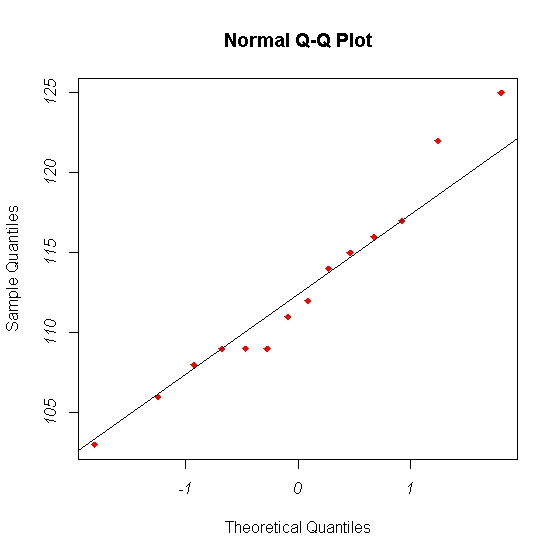
\includegraphics[scale=0.45]{images/Q5examQQplot}
\end{center}

\begin{itemize}
	\item[i.] (1 Mark) Provide a brief description on how to interpret this plot.
	\item[ii.] (1 Mark) What is your conclusion for this procedure? Justify your answer.
\end{itemize}
\newpage
\subsection*{Q5. Testing Normality (3 Marks)} %4 Marks
Consider the following inference procedure performed on data set $X$.
\begin{center}
	\begin{verbatim}
	> shapiro.test(X)
	
	Shapiro-Wilk normality test
	
	data:  X
	W = 0.9619, p-value = 0.6671
	
	\end{verbatim}
\end{center}


\begin{itemize}
	\item[i.] (1 Mark) Describe what is the purpose of this procedure.
	\item[ii.] (1 Mark) What is the null and alternative hypothesis?
	\item[iii.] (1 Mark) Write the conclusion that follows from it.
\end{itemize}

\subsection*{Q6. Testing For Outliers (6 Marks)}
\begin{itemize}
	\item[(i)] (3 Marks) Provide a brief description for three tests from the family of Grubb's  Outliers Tests. Include in your description a statement of the null and alternative hypothesis for each test, any required assumptions and the limitations of these tests.
	\item[(ii)] (3 Marks) Showing your working, use the Dixon Q Test to test the hypothesis that the maximum value of the following data set is an outlier.
	\[ 19,22,23,24,25,26,29,38\]
\end{itemize}

\newpage
\subsection*{Q7. Testing for Outliers (3 Marks)} %4 Marks
The following statistical procedure is based on this dataset.
\begin{center}
\begin{tabular}{|cccc|}
	\hline
	% after \\: \hline or \cline{col1-col2} \cline{col3-col4} ...
	6.98 &8.49 &7.97& 6.64\\
	8.80 &8.48 &5.94& 6.94\\
	6.89 &7.47 &7.32& 4.01\\
	\hline
\end{tabular}
\end{center}

\begin{framed}

	\begin{verbatim}
	> grubbs.test(x, two.sided=T)
	
	Grubbs test for one outlier
	
	data:  x
	G = 2.4093, U = 0.4243, p-value = 0.05069
	alternative hypothesis: lowest value 4.01 is an outlier
	\end{verbatim}
\end{framed}

\begin{itemize}
	\item[i.] (1 Mark) Describe what is the purpose of this procedure. State the null and alternative hypothesis.
	\item[ii.] (1 Mark) Write the conclusion that follows from it.
	\item[iii.] (1 Mark) State any relevant assumptions for this procedure.
\end{itemize}

\subsection*{Q8. Chi-Square Test (9 Marks)} %4 
Suppose you conducted a drug trial on a group of animals and you hypothesized that the animals receiving the drug would show increased heart rates compared to those that did not receive the drug. You conduct the study and collect the following data:
{
	\large
\begin{center}
\begin{tabular}{|c|c|c|c|}
	\hline  & Heart Rate & No Heart Rate  &  \\  
	  & Increased & Increase & Increase \\ 
	\hline Treated  & 36 & 14 & 50 \\ 
	\hline Not Treated & 30 & 25 & 55 \\ 
	\hline  & 66 & 39 & 105 \\ 
	\hline 
\end{tabular} 
\end{center}
}
\begin{itemize}
	\item[i.](1 Mark) Formally state the null and alternative hypotheses.
	\item[ii.] (2 Marks) Compute the cell values expected under the null hypothesis. Show your workings for two cells.
	\item[iii.](3 Marks) Compute the Test Statistic.
	\item[iv.](1 Mark) State the appropriate Critical Value for this hypothesis test.
	\item[v.](2 Marks) Discuss your conclusion to this test, supporting your statement with reference to appropriate values.
\end{itemize}

%\end{itemize}
% -- Part 2 - Hypothesis Testing Computation
%
% 1 Mark
% 1 Mark
%Compute the pooled variance for the aggregate sample
% 1 Mark Standard Error
% 1 Mark Test Statistic
% 1 Mark Appropriate level of significance
% 1 Mark Appropriate degrees of freedom
% 1 Mark Appropriate Critical value
% 1 MArk Discuss your conclusion to this test, supporting your statement with reference to appropriate values.

\newpage


\section*{Formulae and Tables}
\subsection*{Critical Values for Dixon Q Test}
{
	\Large
	\begin{center}
		\begin{tabular}{|c|c|c|c|}
			\hline  N  & $\alpha=0.10$  & $\alpha=0.05$  & $\alpha=0.01$  \\ \hline
			3  & 0.941 & 0.97  & 0.994 \\ \hline
			4  & 0.765 & 0.829 & 0.926 \\ \hline
			5  & 0.642 & 0.71  & 0.821 \\ \hline
			6  & 0.56  & 0.625 & 0.74  \\ \hline
			7  & 0.507 & 0.568 & 0.68  \\ \hline
			8  & 0.468 & 0.526 & 0.634 \\ \hline
			9  & 0.437 & 0.493 & 0.598 \\ \hline
			10 & 0.412 & 0.466 & 0.568 \\ \hline
			11 & 0.392 & 0.444 & 0.542 \\ \hline
			12 & 0.376 & 0.426 & 0.522 \\ \hline
			13 & 0.361 & 0.41  & 0.503 \\ \hline
			14 & 0.349 & 0.396 & 0.488 \\ \hline
			15 & 0.338 & 0.384 & 0.475 \\ \hline
			16 & 0.329 & 0.374 & 0.463 \\ \hline
		\end{tabular} 
	\end{center}
}
\subsection*{Critical Values for Chi Square Test}
{
	\Large
	\begin{center}
		\begin{tabular}{|c|c|c|c|c|}
			\hline 
			n	&	$\alpha=0.10$	&	$\alpha=0.05$	&	$\alpha=0.01$	&	$\alpha=0.001$	\\ \hline
			1	& 	2.705	&	3.841	&	6.634	&	10.827	\\ \hline
			2	&	4.605	&	5.991	&	7.378	&	9.21	\\ \hline
			3	&	6.251	&	7.815	&	9.348	&	11.345	\\ \hline
			4	&	7.779	&	9.488	&	11.143	&	13.277	\\ \hline
			5	&	9.236	&	11.07	&	12.833	&	15.086	\\ \hline
			6	&	10.645	&	12.592	&	14.449	&	16.812	\\ \hline
			7	&	12.017	&	14.067	&	16.013	&	18.475	\\ \hline
			8	&	13.362	&	15.507	&	17.535	&	20.09	\\ \hline
			9	&	14.684	&	16.919	&	19.023	&	21.666	\\ \hline
			10	&	15.987	&	18.307	&	20.483	&	23.209	\\ \hline
		\end{tabular} 
	\end{center}
}
\newpage
\subsection*{Test Statistic for Chi-Square Test}
{
\Large
\[ \chi^2_{TS} = \sum \frac{(\mbox{Observed} -\mbox{Expected} )^2}{\mbox{Expected} }\]
}

\end{document}
\subsection*{Confidence Intervals}
{\bf One sample}
\begin{eqnarray*} S.E.(\bar{X})&=&\frac{\sigma}{\sqrt{n}}.\\\\
S.E.(\hat{P})&=&\sqrt{\frac{\hat{p}\times(100-\hat{p})}{n}}.\\
\end{eqnarray*}
{\bf Two samples}
\begin{eqnarray*}
S.E.(\bar{X}_1-\bar{X}_2)&=&\sqrt{\frac{\sigma^2_1}{n_1}+\frac{\sigma_2^2}{n_2}}.\\\\
S.E.(\hat{P_1}-\hat{P_2})&=&\sqrt{\frac{\hat{p}_1\times(100-\hat{p}_1)}{n_1}+\frac{\hat{p}_2\times(100-\hat{p}_2)}{n_2}}.\\\\
\end{eqnarray*}
\subsection*{Hypothesis tests}
{\bf One sample}
\begin{eqnarray*}
S.E.(\bar{X})&=&\frac{\sigma}{\sqrt{n}}.\\\\
S.E.(\pi)&=&\sqrt{\frac{\pi\times(100-\pi)}{n}}
\end{eqnarray*}
{\bf Two large independent samples}
\begin{eqnarray*}
S.E.(\bar{X}_1-\bar{X}_2)&=&\sqrt{\frac{\sigma^2_1}{n_1}+\frac{\sigma_2^2}{n_2}}.\\\\
S.E.(\hat{P_1}-\hat{P_2})&=&\sqrt{\left(\bar{p}\times(100-\bar{p})\right)\left(\frac{1}{n_1}+\frac{1}{n_2}\right)}.\\
\end{eqnarray*}
{\bf Two small independent samples}
\begin{eqnarray*}
S.E.(\bar{X}_1-\bar{X}_2)&=&\sqrt{s_p^2\left(\frac{1}{n_1}+\frac{1}{n_2}\right)}.\\\\
s_p^2&=&\frac{s_1^2(n_1-1)+s_2^2(n_2-1)}{n_1+n_2-2}.\\
\end{eqnarray*}
{\bf Paired sample}
\begin{eqnarray*}
S.E.(\bar{d})&=&\frac{s_d}{\sqrt{n}}.\\\\
\end{eqnarray*}
{\bf Standard Deviation of case-wise differences (computational formula)}
\begin{eqnarray*}
s_d = \sqrt{ {\sum d_i^2 - n\bar{d}^2 \over n-1}}.\\\\
\end{eqnarray*}
\end{document}
% -- Part 3 - Confidence Interval

% 2 Marks Using previously calculated values, compute the confidence interval
